\documentclass[dvipsnames]{beamer}
\usetheme{metropolis}
\author{Nachiket Namjoshi}
\title{Implementing a Programming Language}
\date{February 18, 2017}
\begin{document}

\begin{frame}
\titlepage
\end{frame}

\section{Introduction}

\begin{frame}{What is A Programming Language?}
\begin{itemize}
\item A \alert{programming language} is basically a set of instructions to be followed by a computer so as to accomplish a particular task.
\end{itemize}
\end{frame}

\begin{frame}{How Does it work?}
\begin{itemize}
\item Computers \emph{do not} understand a programming language.
\item All they do understand is \emph{machine code}.
\item A machine code is a stream of bits (0‘s and 1‘s).
\end{itemize}
\end{frame}
\begin{frame}{So, HOW does it work?}
\begin{figure}
	\includegraphics[scale=0.4]{1}
	\caption{General Compilation}
\end{figure}
\end{frame}

\begin{frame}{What is a Compiler?}
\begin{itemize}
\item Compiler is basically a \alert{software} that converts a programming language into another programming language.
\item This Process is known as \alert{compilation}.
\end{itemize}
\end{frame}


\begin{frame}{Compilation Process}
\begin{figure}
	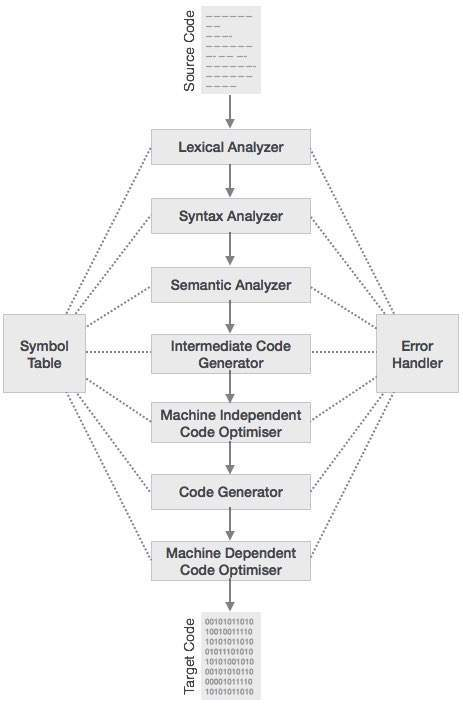
\includegraphics[scale=0.33]{2}
\end{figure}
\end{frame}

\section{Problem Definition}
\begin{frame}{Problem Definition}
To design a compiler that compiles a C program and gives the following output:
\begin{itemize}
\item Pre-processed Code.
\item Equivalent assembly language code
\item Final output of the C program
\end{itemize}
\end{frame}

\section{Proposed System}
\begin{frame}{Software/Hardware Requirements}
Hardware:
\begin{itemize}
\item At \alert{least} a dual core processor
\item Minimum \alert{2GB} RAM
\end{itemize}
Software:
\begin{itemize}
\item Any GNU/Linux Based OS.
\item A C Compiler \emph{(GCC Preferred)}
\end{itemize}
\end{frame}

\begin{frame}{How To Start?}
Steps I followed \emph{(and am following)} while implementation:
\begin{itemize}
\item Plan out the basic approach from start to end
	\begin{itemize}
	\item Separate out all the \alert{lexemes} 
	\item Add them all to an \alert{AST}
	\item Check the syntax
	\item \alert{Emit} proper Assembly code for each statement in the program.
	\end{itemize}
\item Work on each module \alert{one by one}.
\item Integrate all the modules.
\end{itemize}
\end{frame}

\section{Usage and Applications}
\begin{frame}{Applications}
\begin{itemize}
\item Implementing a compiler opens up the scope towards creating/establishing a \emph{\alert{NEW}} programming language.
\item Concepts of Compilers are not limited to Compilers, whereas they are used in \alert{\emph{several}} other fields.
\item Implementing such a significant project gives an \alert{\emph{in-depth}} idea about real life software development.
\end{itemize}
\end{frame}

\begin{frame}{Limitations}
\begin{itemize}
\item The implementation of a compiler is done by several other commercial companies, so it can only be used for educational purposes.
\item A crudely formed compiler \alert{WILL} produced \emph{un-optimised} results.
\item Failing to implement.
\end{itemize}
\end{frame}

\begin{frame} {References}
\begin{itemize}
\item \href{http://digitalcommons.ohsu.edu/cgi/viewcontent.cgi?article=1122&context=csetech}{Abstract syntax in theory and practice}, Eugene J. Rollins
\item \href{http://www.jmodelica.org/api-docs/usersguide/1.6.0/ch11s01.html}{AST Implementation in Python}
\item  Atsushi Yoshida; Yoshinari Hachisu: A Pattern Search Method for Unpreprocessed C Programs Based on Tokenized Syntax Trees, 2014, IEEE 14th Conference.
\item Yoshitaka Kato; Masaya Ozaki; Jun'ya Kani; Nobuhiro Ito; Yoshinobu Kawabe: Developing Compiler for Nihongo Programming Language PEN, 2015, IEEE 15th Conference
\end{itemize}
\end{frame}

\section{THANK YOU}
\end{document}
